\section{\textit{Friends}-method}
\label{sec:method}
Let $C := \{c_1, \dots, c_k\}$, and let $T := \{t_1, \dots, t_n\}$. Without loss of generality, we assume that the elements of $A$~\eqref{eq:adj_matrix} are distances.  
 We will denote the $i$-th row of the matrix $A$ as $\text{row}_i(A)$ and its $j$-th column $\text{col}_j(A)$, i.e.,
\[
\text{row}_i(A) := (a_{i1}, \dots, a_{ik}),
\quad
\text{col}_j(A) := (a_{1j}, \dots, a_{nj}).
\]
In other words, a row $\text{row}_i(A)$ corresponds to the distances between the vertex $t_i$ to all vertices in $C$. A column $\text{col}_j(A)$ corresponds to the distances from a vertex $c_j$ to all vertices in $T$.

In the rest of the text, we assume that all $a_{ij}$ are independent random variables.

Further, under $H_0$ we assume that the attention that each node $c_j$ from $C$ pays to all tags in $T$ is identically distributed. In other words, values in $\text{col}_j(A)$ have the same distribution. We denote it as $P_j$. Typically, all distributions $P_1, \dots, P_k$ are unknown and may vary in nature. 

\subsection*{First step: double ranking}

For each node $c_j \in C$, we rank the elements in the corresponding column $\text{col}_j(A)$ in decreasing order---that is, higher $a_{ij}$ receive lower ordinal numbers. Thus, each entry $a_{ij} $ in $\text{col}_j(A)$ is assigned the ordinal number $o_{ij}$. In cases where multiple entries in $\text{col}_j(A)$ share the same value, we use a randomized tie-breaking procedure.

We denote the matrix containing ordinal numbers $o_{ij}$ as $O$, 
\begin{equation*}
O = \begin{pmatrix}
o_{11} & o_{12} & \dots & o_{1k} \\
 &\cdots & \cdots & \\
o_{n1} & o_{n2} & \dots & o_{nk}
\end{pmatrix}, 
\quad
o_{ij} :=\text{rank}\left(a_{ij}~ \text{inside}~\text{col}_j(A)\right).
\end{equation*}
As before, we denote the $i$-th row of $O$ as $\text{row}_i(O) := (o_{i1}, \dots, o_{ik})$.

Next, we decreasingly order the ranks stored in $\text{row}_i(\mathcal{O})$. Denote the corresponding rearrangement as $r_{i1}, \dots, r_{ik}$. By construction, $r_{i1} \le r_{i2} \le \dots \le r_{ik}$. Let the corresponding matrix be
\begin{equation}
\label{def:R}
R = \begin{pmatrix}
r_{11} & r_{12} & \dots & r_{1k} \\
 &\cdots & \cdots & \\
r_{n1} & r_{n2} & \dots & r_{nk}
\end{pmatrix}.
\end{equation}

\paragraph{Idea behind the statistical test} To find the best friends of the tag $t_i$ we are going to split the items inside $\text{row}_{i}(\mathcal{R}) = (r_{i1}, \dots, r_{ik})$ into two non-intersecting groups. One group will match best friends and the other group will match all other nodes. 

%NB! Сказать в дискуссии, что метод работает даже если модельное предположение ломается?
\subsection*{Second step: statistical test}
Keeping in mind that now we deal with a single tag $t_i$, let's, for simplicity, omit index $i$. \textcolor{red}{Then,} 
\[
\text{row}_{i}(\mathcal{R}) = (r_{1}, \dots, r_{k}), 
\quad
r_{1} \le \cdots \le r_{k}.
\]

Before proceeding, we must verify that the tag is not indifferent to all nodes, e.g. to reject $H_0$. To do this, one can either use a test to assess the homogeneity of the sample $r_{1}, \cdots, r_{k}$ or, alternatively, apply an information criterion, which will be introduced later in the text (see paragraph \textit{Information Criterion})

Assuming a tag has at least one true friend, we aim to split all nodes into two groups. A group containing best friends nodes, i.e. the nodes corresponding to $r_1, \dots, r_{s^*}$ and all the other.

Before introducing a statistical model, we recall two important facts. First, $r_{1}, \cdots, r_{k}$ are independent random variables. Second, each $r_l$ ($1\le l \le k$) takes value ranging from $1$ to $n$. This is because, by construction, each $r_l$ is an ordinal number.

Under $H_1$, we assume that each $r_l$ ($1\le l \le k$) comes from a mixture of two uniform distributions on the discrete grid $1, \dots, n$.
Specifically, the mixture consists of a uniform distribution supported on $1, \dots, m^*$, and a uniform distribution supported on $m^* + 1, \dots, n$, where $m^*$ is an unknown parameter. The probability of each $r \in \{1, \dots, m^*\}$ is $\frac{p^{*}}{m^*}$ and $r \in \{ m^*+1, \dots, n\}$ is $\frac{1 - p^{*}}{n - m^*}$,
see Fig.\ref{fig:model}.
\begin{figure}
 \centering
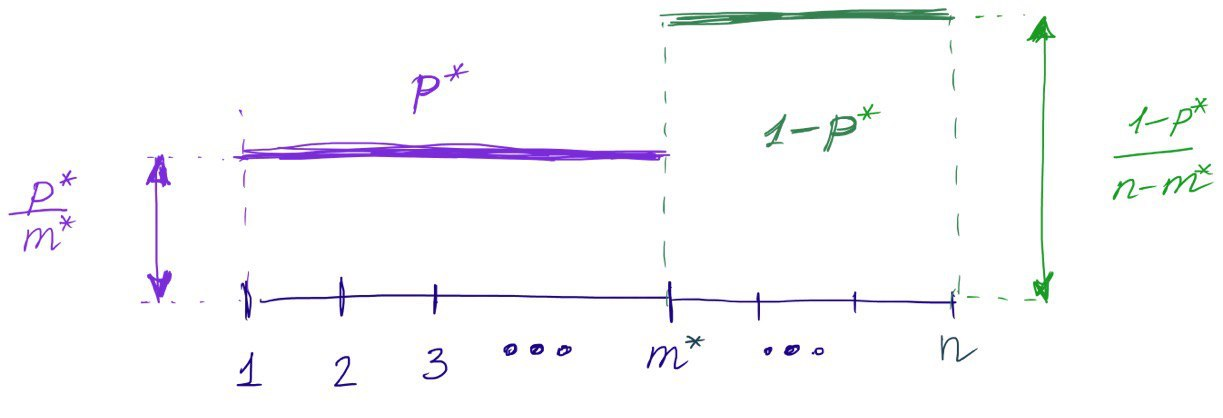
\includegraphics[width=0.8\textwidth]{model.jpeg}
 \caption{....}
 \label{fig:model}
\end{figure}

Note, that $p^*$ and $m^*$ are not known.
We use the maximum likelihood estimation to estimate them based on the observed data $r_1, \dots, r_k$. The likelihood of the mixture is
\[
L(p, m; r_1, \dots, r_k) := s\ln\left(\frac{p}{m}\right) + (k-s)\ln\left(\frac{1-p}{n - m}\right),
\quad
s: r_{s} \le m, ~r_{s+1} > m.
\]
The goal is to find $\hat{p}$ and $\hat{m}$ maximizing $L(p, m; r_1, \dots, r_k)$. Optimizing by $p$ ensures that $\hat{p} = \frac{s}{k}$. All aforementioned ensures that one can use brute-force search over $m$ to find the optimal parameters.

\paragraph{Information criterion}
One can avoid using the homogeneity test by applying the following information criterion.
The approach relies on some preliminary knowledge of the data. Specifically, one has to assume how likely it is that the tag $t$ has friends. We denote the corresponding probability as $q \in (0, 1)$ and set
\[
L_1 := L(\hat{p}, \hat{m}) + \ln(q),
\quad
L_2 := L(0, 0) + \ln(1-q).
\]
The best fit corresponds to $\max\{L_1, L_2\}$.

